\begin{frame}
    \centering
    \Huge \textcolor{blue3}{SQL}

\end{frame}

\begin{frame}
	
	\frametitle{Motivación. Estadística en EEUU}
	
	\begin{figure}[h]
		\centering
		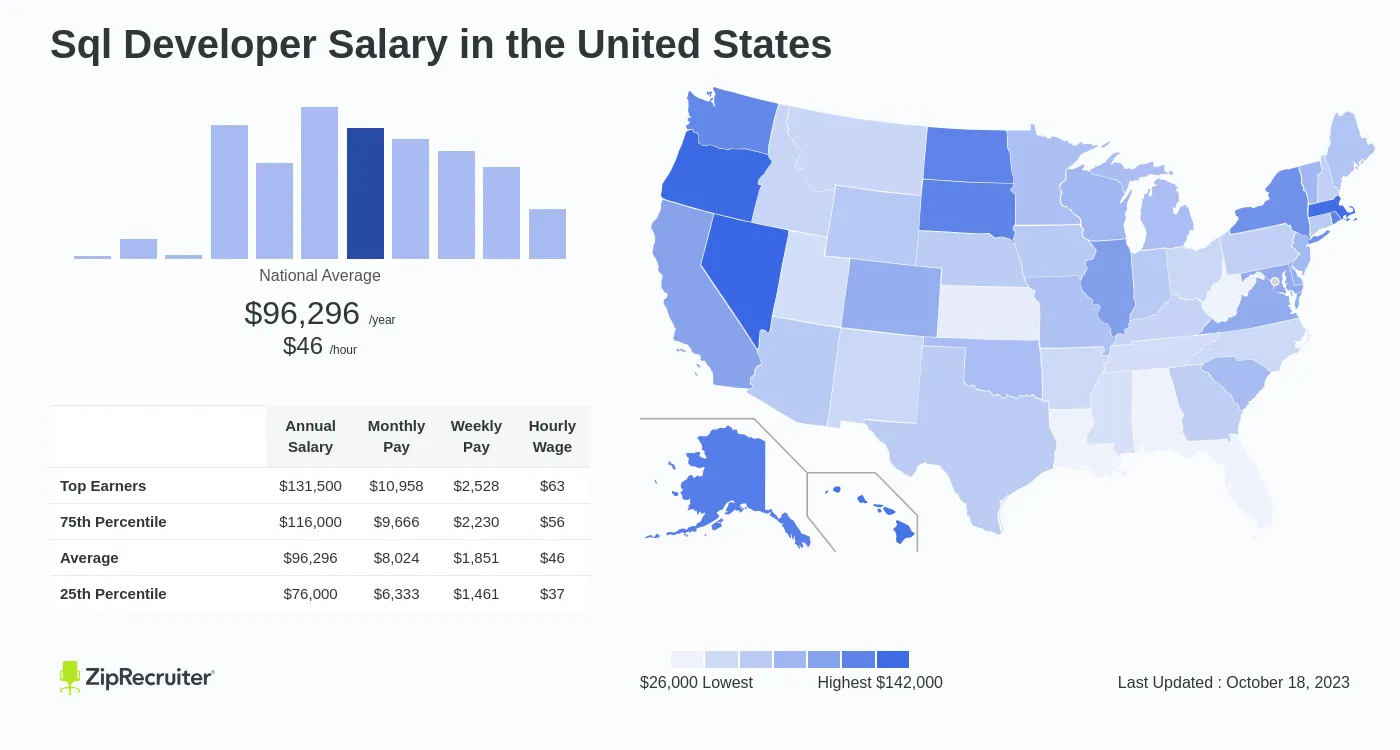
\includegraphics[scale=0.25]{sql-developer-salary.png}
	\end{figure}
	
\end{frame}

%------------------------------------------------

\begin{frame}
	
	\frametitle{Motivación. Estadística en EEUU}
	
	\begin{figure}[h]
		\centering
		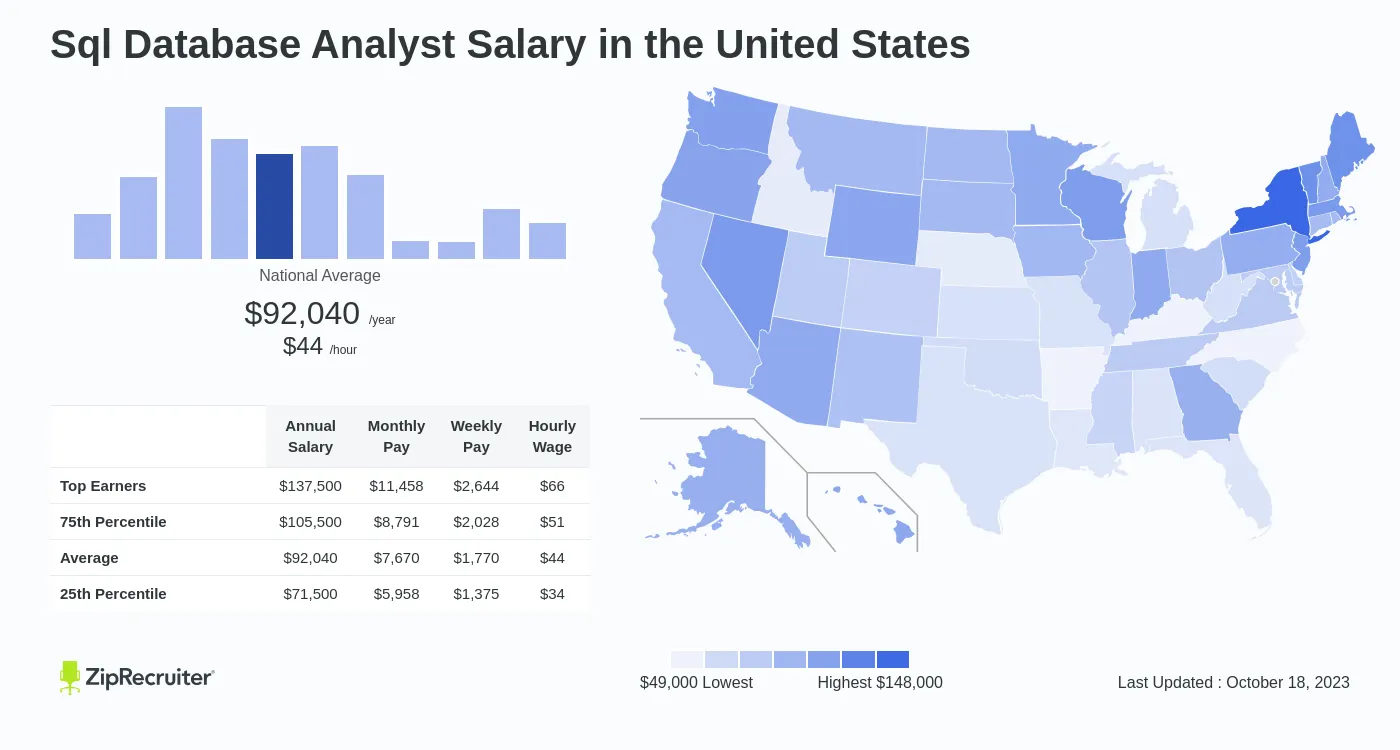
\includegraphics[scale=0.25]{sql-database-analyst-salary.png}
	\end{figure}
	
\end{frame}

%------------------------------------------------

\begin{frame}
	
	\frametitle{Motivación. Estadística en EEUU}
	
	\begin{figure}[h]
		\centering
		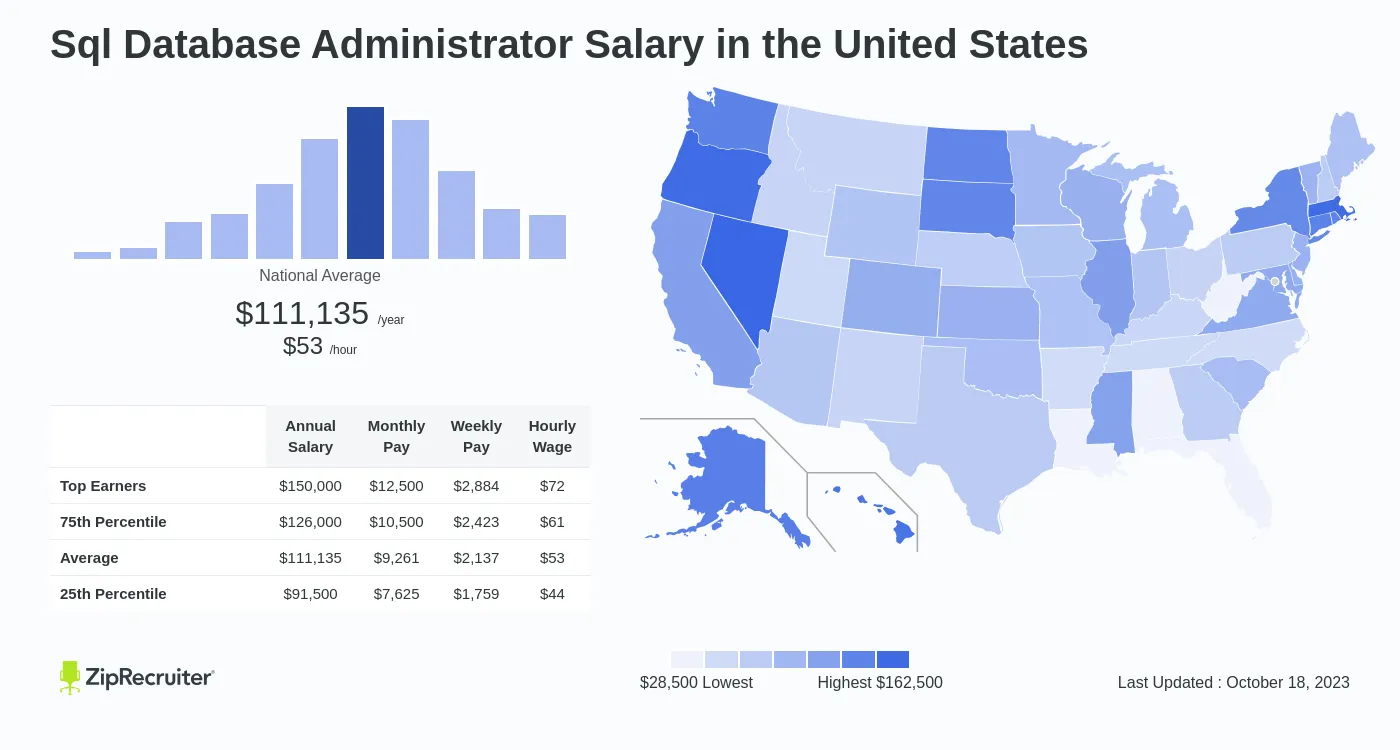
\includegraphics[scale=0.25]{sql-database-administrator-salary.png}
	\end{figure}
	
\end{frame}

%------------------------------------------------

\begin{frame}

	\frametitle{Fundamentos de SQL}
	
	\begin{center}
		\textbf{SQL} 
	
		Structured Query Language
	\end{center}
	
	\pause
	
	\begin{itemize}[<+->]
	
		\item Lenguaje de consulta dise\~nado espec\'ificamente para trabajar con bases de datos relacionales
		\item Lenguaje declarativo
		\item Desarrollado a partir de la década de 1970 por IBM, posterior a la definición del modelo relacional
		\item Desde su creaci\'on, se ha estandarizado a tal punto que es el lenguaje base de muchos otros Sistemas de Gestión de Bases de Datos (MySQL, SQL Server, MS Access, Oracle, Sybase, Informix, Postgres)

	\end{itemize}
	
	\note<5>{@NOTE
		Pudiese decir que es el lenguaje que más se utiliza, puesto que todos los sistemas, independiente de la tecnología que use, si trabaja con base de datos relacionales, es muy probable que use directa o indirectamente SQL.
		
		Es un lenguaje maduro, basado en el álgebra relacional, con poca discrepancias entre sus versiones. Es muy requerido en la vida laboral. 
		
		Si analizamos ciertos aspectos, podemos entender porqué no es un lenguaje de programación. 
		- enfocado en datos, no en operaciones. Sirve para definir, manipular y acceder a los datos almacenados en bases de datos.
		- no puede realizar tareas propias de la programación como bucles, condicionales, declaración de variables, etc.
		- no permite abstraer la lógica de negocio en objetos, clases y métodos como en la programación orientada a objetos.
		- es un estándar implementado por diferentes motores de bases de datos, no un lenguaje de programación como Java, Python, etc.
		- se utiliza en combinación con lenguajes de programación para acceder y gestionar bases de datos desde aplicaciones externas.
	}

\end{frame}

%------------------------------------------------

\begin{frame}

	\frametitle{Componentes de SQL}
	
	
	\begin{itemize}
	
		\item Catálogo de datos

	\end{itemize}
	
	\begin{figure}[h]
		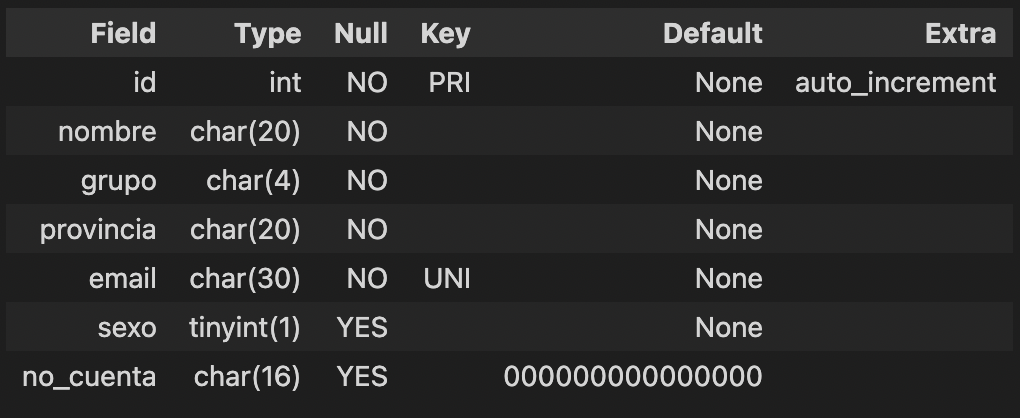
\includegraphics[scale=0.45]{describe.png} Descripción de la tabla
		Datos de la tabla 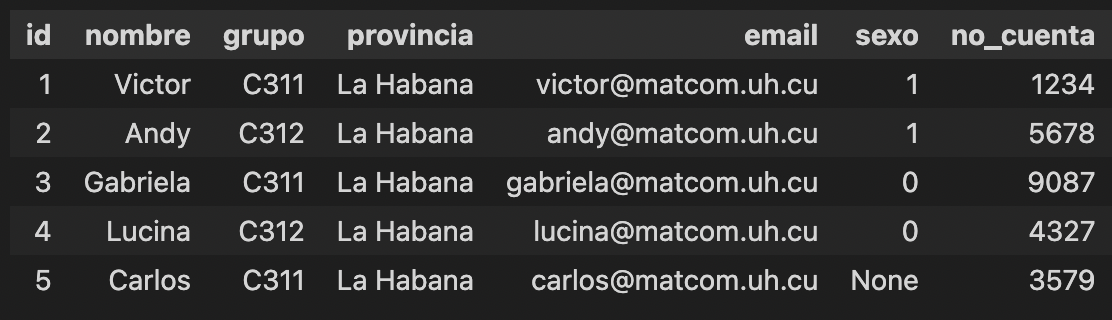
\includegraphics[scale=0.45]{datos.png} 
	\end{figure}

\end{frame}


%------------------------------------------------

\begin{frame}
	
	\frametitle{Componentes de SQL}
	
	
	\begin{itemize}
		
		\item Comandos u órdenes
		\begin{itemize}
			\item<2-> Palabras o frases reservadas: $FROM$, $PRIMARY\ KEY$
			\item<3-> Constantes numéricas y literales.
			\item<4-> Variables: Nombre de tablas y atributos
			\item<5-> Operadores: 

			\only<6->{
			\begin{itemize}
				\item Numéricos: $-$, $+$, $*$
				\item Lógicos: $AND$, $OR$, $NOT$
				\item Relacionales: $<$, $<=$, $>=$, $>$, $=$, $<>$
				\item De cuantificación: $ALL$, $ANY$, $EXIST$
			\end{itemize}
			}
			
		\item<7-> Claúsulas específicas: $BETWEEN$, $IN$, $LIKE$, $DISTINCT$, $IS\ NULL$
		\item<8-> Funciones propias ($SUM$, $IFNULL$) y creadas por el desarrollador
		\item<9-> Restricciones de integridad: $FOREIGN\ KEY$
			
		\end{itemize}
		
	\end{itemize}
	
\end{frame}

%------------------------------------------------

\begin{frame}
	\frametitle{Tipos de comandos}
	
	\begin{tikzpicture}[
		scale=0.75,
		transform shape,
        		mindmap,
        		concept color = blue!40,
        		every node/.style = {concept},
        		grow cyclic,
        		level 1/.append style = {
            		concept color = blue!25,
           		level distance = 4.5cm,
            		sibling angle = 120
        		},
       		level 2/.append style = {
            		concept color = blue!10,
            		level distance = 3cm,
            		sibling angle = 45
        		}
    	]
    	\node [concept] at (current page.center) {\textbf{Concepto} \\ Palabra reservada o sintaxis}
    	child[grow=190]{
        		node {\textbf{DDL} \\ Lenguaje de Definici\'on de Datos}
		child[grow=175]{node {Create}}
		child[grow=140]{node {Alter}}
		child[grow=105]{node {Drop}}
		child[grow=70]{node {Truncate}}
         }
         child[grow=230]{
         	node {\textbf{DML} \\ Lenguaje de Manipulaci\'on de Datos}
         	child[grow=200]{node {Insert}}
         	child[grow=235]{node {Update}}
         	child[grow=270]{node {Delete}}
         }
         child[grow=280]{
        		node {\textbf{DQL} \\ Lenguaje de Consulta de Datos}
		child[grow=310]{node {Select}}
         }
         child[grow=340]{
        		node {\textbf{DCL} \\ Lenguaje de Control de Datos}
		child[grow=315]{node {Revoke}}
		child[grow=280]{node {Grant}}
         }
         child[grow=20]{
        		node {\textbf{TCL} \\ Lenguaje de Control de \\ Transacciones}
		child[grow=0]{node {Rollback}}
		child[grow=325]{node {Commit}}
         }
        ;
	\end{tikzpicture}
	
	\note{@NOTE
		DDL se refiere a comandos SQL que diseñan la estructura de la base de datos.
		DQL consiste en instrucciones para recuperar datos almacenados en bases de datos relacionales.
		DML escriben información nueva o modifican los registros existentes en una base de datos relacional.
		DCL  administra o autoriza el acceso a la base de datos.
		TCL hace cambios en la base de datos de manera automática. 
	}

\end{frame}

%------------------------------------------------

\begin{frame}

	\frametitle{Jugando con SQL}
	
	Auxiliarse del fichero \alert{Conferencia\_6.ipynb} % @TODO cambiar nombre


\end{frame}

%------------------------------------------------

\begin{frame}

	\frametitle{Tipos de datos}

	\begin{columns}[c] 
		\begin{column}{0.45\textwidth} % Left column width
			\begin{itemize}
	
				\item<2-> Numéricos
				\only<2->{
					\begin{itemize}
					\item INT
					\item BIT o BOOLEAN
					\item MONEY
					\item FLOAT
				\end{itemize}
				}
			
			\item<3-> Cadenas de caracteres
				\only<3->{
				\begin{itemize}
					\item CHAR o NCHAR
					\item VARCHAR o NVARCHAR
			\end{itemize}

				}
			
			\item<4-> Cadenas binarias
			\only<4->{
				\begin{itemize}
					\item BINARY
				\end{itemize}

			}
			
		\end{itemize}
		\end{column}
		
		\begin{column}{0.5\textwidth} % Right column width
		\begin{itemize}
		
			\item<5-> Fecha y hora
			\only<5->{
			\begin{itemize}
				\item DATE				
				\item TIME
				\item DATETIME
			\end{itemize}
			}
			
			\item<6-> Otros
			\only<6->{
			\begin{itemize}
				\item XML				
				\item GEOGRAFÍA ESPACIAL
			\end{itemize}

			}
			
		\end{itemize}			
		\end{column}
		
	\end{columns}

	\vspace{5mm}

	\centering
	\only<7->{
	\Large \textcolor{red}{Consultar manual de SQL}
	}

\end{frame}

%------------------------------------------------

\begin{frame}

	\frametitle{Restricciones de integridad}
	
	\note{@NOTE
		- Reglas y restricciones predefinidas, muchas veces a raíz de las reglas del negocio. 
		- Se aplican por columna.
		- La operación de inserción se efectúa, solo si se cumple todas las restricciones definidas.
		- 
	}
	
	\begin{itemize}
		\item<2-> PRIMARY KEY
		\item<3-> FOREIGN KEY	
		\only<3->{
			\begin{itemize}
				\item Activadores: ON UPDATE, ON DELETE
				\item Modificadores: CASCADE, RESTRICT, SET NULL, SET DEFAULT, NO ACTION
			\end{itemize}
		}
		
		\item<4-> NOT NULL 
		\item<5-> UNIQUE
		\item<6-> CHECK \textit{condici\'on}
		\item<7-> DEFAULT	\textit{valor}
	
	\end{itemize}
	
	

\end{frame}

%------------------------------------------------

\begin{frame}
	
	\frametitle{Dudas, comentarios, sugerencias}
	
	\begin{figure}[h]
		
\includegraphics[scale=0.4]{duda.jpg}
	\end{figure}
	
	

\end{frame}